\chapter{Riemann积分}

\section{Riemann可积的定义}

我们先来看一个例子: 尝试计算(定义)抛物线$y=x^2,0\leq x \leq 1$与$x$轴围成的面积. 一种自然的思路是利用矩形进行逼近, 因为我们可以简单地定义出矩形的面积. 具体来说, 考虑$[0,1]$区间的一个分割$\pi = \{ 0=x_0<x_1<\cdots <x_{n-1}<x_n=1 \}$, 并在每个小区间内部取点$\xi _i \in [x_{i-1},x_i]$, 记$\xi = \{ \xi _1,\cdots ,\xi _n \}$. 我们希望定义如下的极限就是所求面积: $$\lim_{\| \pi \| \to 0} \sum_{i=1}^{n}(x_i-x_{i-1})\xi _i^2. $$
其中, 极限过程$\| \pi \| \to 0$的意思是$\max_{1\leq i \leq n} \{x_i-x_{i-1}\} \to 0$(这的确构成一种极限过程, 后面会证明). 

这种定义有非常明显的问题: 
\begin{itemize}
	\item 分割$\pi$和标记点$\xi$并不确定, 因而无法很方便地计算这个极限. 
	\item 由于不便将该式化简, 我们甚至不知道这样的极限是否存在. 
\end{itemize}
针对这两个问题, 可能会有如下想法: 
\begin{itemize}
	\item 用平均分割和统一的标记点选取标准来代替一般化的方法. 注意这种计算方式一定是充分条件. 
	\item 类似于数列, 既然难以判断极限是否存在, 可以考虑定义上下极限来逼近. 
\end{itemize}
综合这两种想法, 在本例中我们可以如下考察所求的面积: 首先取平均分割$\pi_{n}=\{ x_i=\frac{i}{n} \}$, 接着选择两种不同的标记点集$\displaystyle\xi _L = \big\{ \xi _i :  \xi _i ^2= \inf_{x_{i-1} \leq x \leq x_i} x^2 \big\}$, $\displaystyle\xi _U = \big\{ \xi _i : \xi _i ^2= \sup_{x_{i-1} \leq x \leq x_i} x^2 \big\}$. 考虑极限过程$n\to \infty$, 于是两种极限$S_L$和$S_U$就是: $$S_L = \lim_{n\to \infty} \left( \frac{1}{n} \sum_{i=1}^{n} \frac{(i-1)^2}{n^2} \right) = \lim_{n\to \infty} \frac{2n^2-3n+1}{6n^2} = \frac{1}{3} ,  $$
$$S_U = \lim_{n\to \infty} \left( \frac{1}{n} \sum_{i=1}^{n} \frac{i^2}{n^2} \right) = \lim_{n\to \infty} \frac{2n^2+3n+1}{6n^2} = \frac{1}{3}.$$
注意到$S_L=S_U = \frac{1}{3}$, 于是所求面积(似乎)就是$\frac{1}{3}$. 

上面的例子就是利用Riemann和进行逼近计算(定义)的做法. 我们不难想到另一种方法: 先定义所谓阶梯函数(这种函数的积分易于定义), 再考虑找到特定函数的阶梯函数逼近, 最后计算极限阶梯函数的积分即可. 这两种方法本质上是相同的, 只是操作顺序不一样. 然而利用后者有两个优势: 我们能够自然地理解Riemann积分的某些缺陷(例如只能处理有界函数), 另外实际上Riemann和的定义无法推广到$\R ^n$上(依赖序关系). 


\subsection{阶梯函数及其积分}

首先我们考虑\textit{示性函数}(characteristic function): 设$E \subseteq \R$, 则定义$$\chi _{E}:\R \to \{ 0,1 \},\quad \chi _{E} (x) = \begin{cases}
	1 & x \in E \\ 0 & x \notin E
\end{cases}.$$
我们希望定义$\chi _E$的积分, 而这自然需要定义集合$E$的长度. 我们不希望引入繁杂的测度理论, 于是承认下方的“公理”: 对于某个将集合映射到其对应长度的函数$\mu$, 我们希望有$$\mu ((a,b)) = \mu ([a,b]) = \mu ([a,b)) = \mu ((a,b]) = b-a, $$
$$\mu ((-\infty ,+\infty)) = \mu ((-\infty ,b)) = \mu ((a ,+\infty)) = +\infty .$$
第一行的“公理”也在告诉我们: 像$a,b$这样的点是没有长度的. 

于是, 我们可以定义示性函数的\textit{积分}(integral)为$$\int \chi _E := \mu (E). $$
特别地, $$\int \chi _{(a,b)} = \int \chi _{[a,b]} = \int \chi _{[a,b)} = \int \chi _{(a,b]} = b-a. $$
当然, 实际定义阶梯函数的积分时只需要用到$E$是区间的情况, 因此上方不严谨的思考并不影响结果的正确性. 

接下来看\textit{阶梯函数}(更多时候称为\textit{简单函数}, simple function): 

\begin{definition}{分划, 阶梯函数, 阶梯函数的积分}
	设闭区间$I=[a,b]$. 
	\begin{itemize}
		\item 称形如$$\pi = \{ a=x_0<x_1<\cdots <x_{n-1}<x_n=b \}$$
		的集合为$I$的一个\textit{分划}(partition). 
		\item 定义分划$\pi$的\textit{步长}(step): $$\| \pi \| := \max_{1 \leq i \leq n} \{ x_i-x_{i-1} \}. $$
		\item 对于分划$\pi= \{ a=x_0<\cdots <x_n=b \}$, 称形如$$f = \sum_{i=1}^{n} \lambda _i \chi _{(x_{i-1},x_{i})} $$
		(其中$\lambda _i \in \R$)的函数为$\pi$上的一个\textit{阶梯函数}. 记$I$上全体阶梯函数的集合为$\mathcal{S}(I)$. 
		\item 承上一条, 定义$f$的\textit{积分}(integral)为$$\int f := \sum_{i=1}^{n} \lambda _i \int \chi _{(x_{i-1},x_i)} = \sum_{i=1}^{n} \lambda _i (x_i-x_{i-1}). $$
	\end{itemize}
\end{definition}
\begin{remark}
	刚才说过, 点是没有长度的, 因此阶梯函数在分割点处的取值应当对最终结果没有影响. 
\end{remark}
\begin{remark}
	为了避免与原函数的符号相混淆, 也记$\int f = \int _I f = \int_a^b f$. 不过为了方便, 我们暂时混用这些符号. 
\end{remark}

这里, 我们实际上需要验证阶梯函数积分的良定义性. 也就是说, 如果$\pi, \pi '$均与$f$相容, 则$f$依这两种分划的积分相等. 一般地, 我们称$\pi ' \prec \pi$($\pi '$比$\pi$细), 如果$\pi$的分割点都是$\pi '$的分割点. 于是我们只需要验证, 若$\pi ' \prec \pi$, 则$f$依这两种分划的积分相等(这是因为我们可以取$\overline{\pi} = \pi \cup \pi '$). 而这是显然的. 

接下来研究积分算子的性质: 

\begin{proposition}{阶梯函数积分算子的性质}
	设闭区间$I=[a,b]$. 设$f,g \in \mathcal{S}(I)$. 则$\int : \mathcal{S}(I) \to \R$满足: 
	
	a) 线性: $$\int (\lambda f+ \mu g) = \lambda \int f + \mu \int g.$$
	
	b) 区间可加性: 设$I=[a,c] \cup [c,b]$, 则$$\int_a^b f = \int_a^c f + \int_c^b f. $$
	
	c) 三角不等式: $$\left| \int f \right| \leq \int |f|. $$
	
	d) 保号性/保序性: 若$f \geq 0$, 则$$\int f \geq 0. $$
	\qquad 特别地, 若$f \leq g$, 则$$ \int f \leq  \int g.$$
	
	e) 对积分的估计: 选取与$f$相容的分划$\pi= \{ a=x_0<\cdots <x_n=b \}$后, $$\left| \int_a^b f \right| \leq |b-a| \sup_{1 \leq i \leq n} |\lambda _i|. $$
\end{proposition}
\begin{proof}
	注意到阶梯函数是有限求和, 诸命题的验证就是显而易见的了. 
\end{proof}

\subsection{Riemann可积的定义}

现在来对一般函数定义Riemann积分. 首先是从阶梯函数角度出发: 

\begin{definition}{Riemann可积}
	设闭区间$I=[a,b]$. 称$f$是\textit{Riemann可积的}, 如果对任意$\varepsilon >0$均存在$F,e \in \mathcal{S}(I)$使得$$\forall x \in I,|f(x)-F(x)|<e(x),\qquad \int e < \varepsilon .$$
	全体$I$上Riemann可积的函数构成集合$\mathcal{R}(I)$. 
\end{definition}


我们需要对上述定义中的$F$逐个求积分并取其“极限”. 从上方的定义, 我们不难想到类似于序列逼近函数极限的思路: 考虑某种意义上的一列逼近函数$\{ f_n \}$, 然后定义$$\int f := \lim_{n\to \infty} \int f_n.$$

\begin{proposition}{} \label{pro:jptihjuudgjxdkyi}
	设闭区间$I=[a,b]$. 则下列说法等价: 
	\begin{itemize}
		\item $f$是Riemann可积的. 
		\item 存在阶梯函数序列$\{ f_n \},\{ e_n \}$使得$$\forall x \in I,|f(x)-f_n(x)|<e_n(x),\qquad \lim_{n\to \infty} \int e_n = 0.$$
		并且令$$\int f := \lim_{n\to \infty} \int f_n .$$
	\end{itemize}
\end{proposition}
\begin{proof}
	1) $\Rightarrow$ 2): 对任意$n>0$, 存在$f_n$使得$|f(x)-f_n(x)|<e_n(x)$使得$\int e_n < 1/n$, 从而$\lim_{n\to \infty} \int e_n = 0$. 

	2) $\Rightarrow$ 1): 显然. 

	另外, 我们还需证明$\int f = \lim_{n\to \infty} \int f_n$是良定义的, 即极限存在且不依赖于$\{ f_n \}$的选取: 

	由于$|f_n(x)-f_m(x)| \leq |f(x)-f_n(x)| + |f(x)-f_m(x)| \leq e_n(x)+e_m(x)$, 在两边积分可得$$\left| \int f_n-\int f_m \right| \leq \int |f_n-f_m| \leq \int e_n + \int e_m \to 0.$$
	这说明$\{ \int f_n \}$是Cauchy列, 进而存在极限. 

	另一方面, 设有另外的$\{ f'_n \}$和$\{ e'_n \}$符合要求, 则$|f_n(x)-f'_n(x)| \leq |f(x)-f_n(x)| + |f(x)-f'_n(x)| \leq e_n(x)+e'_n(x)$, 两侧积分可得$$\left| \int f_n - \int f'_n \right| \leq \int |f_n-f'_n| \leq \int e_n+ \int e'_n \to 0.$$
	于是两个极限相等. 
\end{proof}


类似于阶梯函数积分算子的性质, 对一般的积分算子也有如下性质: 

\begin{proposition}{} \label{pro:jiffxkvi1}
	设闭区间$I=[a,b]$. 设$f,g \in \mathcal{R}(I)$. 则$\int : \mathcal{R}(I) \to \R$满足: 
	
	a) 线性: $$\int (\lambda f+ \mu g) = \lambda \int f + \mu \int g.$$
	
	b) 区间可加性: 设$I=[a,c] \cup [c,b]$, 则$$\int_a^b f = \int_a^c f + \int_c^b f. $$
	
	c) 三角不等式(注意这依赖于$|f|$的可积性, 当然证明是显然的): $$\left| \int f \right| \leq \int |f|. $$
	
	d) 保号性/保序性: 若$f \geq 0$, 则$$\int f \geq 0. $$
	\qquad 特别地, 若$f \leq g$, 则$$ \int f \leq  \int g.$$
	
	e) 对积分的估计: 选取与$f$相容的分划$\pi= \{ a=x_0<\cdots <x_n=b \}$后, $$\left| \int_a^b f \right| \leq |b-a| \sup_{a \leq x \leq b} |f(x)|. $$
\end{proposition}
\begin{remark}
	尽管无法给出$\int fg$关于$\int f,\int g$的表达式, 我们仍然希望证明$fg$是可积的. 然而, 正是由于$\int fg$不好表示, 这里无法证明. 在下一节我们会处理这个问题. (实际上用阶梯函数的确能处理, 只不过太麻烦)
\end{remark}

接着从Riemann和角度出发. 类似于前文的例子, 如下定义: 基于分割点集$\pi$和标记点集$\xi$, 则$f$的\textit{Riemann和}为: $$S(f;\pi ,\xi) := \sum_{i=1}^{n} (x_i-x_{i-1})f(\xi _i) .$$
对于取定的函数$f$, 定义它的基为$\mathcal{B} := \{ B_{\delta}:\delta >0 \}$, 其中$B_{\delta} := \{ (\pi ,\xi) : \| \pi \|< \delta \}$. 不难证明, 这的确是一个基. 

\begin{proposition}{}
	设闭区间$I$, $f$在$I$上Riemann可积, 则
	\begin{center}
		$\displaystyle \lim_{\mathcal{B}} S(f;\pi ,\xi) = \int_I f.$
	\end{center}
\end{proposition}
\begin{proof}
	任取$\varepsilon >0$, 设阶梯函数$F,e$使得$|f(x)-F(x)|<e(x)$且$\int e(x) < \varepsilon$, 且不妨设$F,e$的分割点集均为$\pi _0 =\{ a=x_0<\cdots <x_n=b \}$. 待定分割点集$\pi = \{ a=y_0<\cdots <y_m=b \}$和与之对应的任意标记集$\xi$. 令$\| \pi \| < \min_{1 \leq i \leq n} \{ x_i-x_{i-1} \}$, 于是$$\left| S(f;\pi ,\xi) - \int_I f \right| \leq \sum_{i=1}^{m} \left| f(\xi _i)-\int_{y_{i-1}}^{y_i} f \right|. $$
	我们基本的思路是控制住$|(y_i-y_{i-1})f(\xi _i)-\int_{y_{i-1}}^{y_i}|$. 比较容易的方法是将$|f(x)|$放缩为其上界$M$, 从而该式不超过$2M(y_i-y_{i-1})$. 然而, 若将其累加, 最后无法得到可用$\| \pi \|$控制的极限. 因此, 希望这种(无可奈何的)放缩尽可能少. 特别地, 注意到那些使得$(y_{i-1},y_i) \subseteq (x_{j-1},x_j)$的区间可用$\varepsilon$放缩, 而剩下的区间不超过$n$个(为什么?), 这些区间采用刚才的放缩就是可以容忍的. 因此, 对$i$, 分情况讨论: 
	
	若$(y_{i-1},y_i)$完全包含在某个$(x_{j-1},x_j)$中: 易知$|f(x)-f(\xi _i)| \leq |f(x)-F(x)| + |F(\xi _i)-f(\xi _i)| \leq e(x)+e(\xi _i)$, 
	从而$$\left| (y_i-y_{i-1})f(\xi _i)-\int_{y_{i-1}}^{y_i} f \right| \leq 2\int_{y_{i-1}}^{y_i} e.$$
	
	若$(y_{i-1},y_i)$恰包含某个$x_j$: 由$f$可积知$f$有界, 设$|f(x)|<M$. 此时有$$\left| (y_i-y_{i-1})f(\xi _i)-\int_{y_{i-1}}^{y_i} f \right| \leq 2(y_i-y_{i-1})M \leq 2\| \pi \|M.$$
	
	综上可得, $$\left| S(f;\pi ,\xi) - \int_I f \right| \leq 2\sum_{i=1}^{m} \int_{y_{i-1}}^{y_i} e + 2n\| \pi \|M \leq 2\varepsilon + 2nM\| \pi \|.$$
	先令$\| \pi \|\to 0$, 则$\limsup_{\| \pi \|\to 0} LHS \leq 2\varepsilon$. 再令$\varepsilon \to 0$即得. 
\end{proof}


\subsection{非负函数的积分, 连接阶梯函数与Riemann和的途径}

从坐标图上来看, 将$f$拆分为非负部分$f^+$和非正部分$f^-$再分别计算两部分的积分似乎是一个可行的方法, 即令$f=f^+-f^-$, 之后定义非负函数$g$的积分为$$\int g := \sup \left\{ \int G:0\leq G \leq g, G \in \mathcal{S}(I)  \right\}, $$
最后令$\int f = \int f^+ - \int f^-$. 

我们先来研究最简单的情形, 即$f$本身就是非负函数: 

\begin{proposition}{} \label{pro:fwfuhjuubijb}
	设闭区间$I=[a,b]$, $f \geq 0$. 则在下列说法中, 1)可以推出2), 而2)加上条件$$\sum_{i=1}^{\ell} \omega (f,(x_{i-1},x_i)) (x_i-x_{i-1}) \to 0,\quad \| \pi \| \to 0$$可以推出1). 
	\begin{itemize}
		\item $f$是Riemann可积的. 
		\item $f$有界, 则集合$$\mathcal{A} = \left\{ \int F:0\leq F \leq f, F \in \mathcal{S}(I)  \right\}$$
		有界. 进而$\sup \mathcal{A}$存在, 令$$\int f := \sup \mathcal{A}.$$
	\end{itemize}
\end{proposition}
\begin{proof}
	(1) 应用上个命题的等价条件, 由于阶梯函数都有界, 显然$f$有界. 下证$\lim_{n\to \infty} \int f_n = \sup \mathcal{A}$. 假设该式不成立, 即存在$M,\varepsilon$使得$\lim_{n\to \infty} \int f_n < M < M+\varepsilon < \sup \mathcal{A}$, 于是对足够大的$n$均有$\int f_n < M$, 且存在阶梯函数$0\leq F \leq f$使得$\int F > M+\varepsilon$. 这就是说, $$e_n(x) > f(x)-f_n(x) \geq F(x)-f_n(x).$$
	两侧(均为非负的阶梯函数)同时积分, 即得$\int e_n(x) \geq \int F(x) - \int f_n(x) > \varepsilon >0$, 矛盾. 因此$\lim_{n\to \infty} \int f_n = \sup \mathcal{A}$. 
	
	(2) 对于$\mathcal{S}(I) \ni F,F' \geq 0$, 定义$F,F'$等价当且仅当它们的分割点集是一样的. 在每个等价类$[F]$中, 设分割点集为$\pi$, 定义该等价类的“极大项”为$$\varphi ([F]) := \sum_{i=1}^{n} \inf_{(x_{i-1},x_i)} f \cdot \chi _{(x_{i-1},x_i)}.$$
	显然$\tilde{\mathcal{A}}:=\{ \int \varphi ([F]):\mathcal{S}(I) \ni F \geq 0 \}$是$\mathcal{A}$的子集, 且$\sup \tilde{\mathcal{A}} = \sup \mathcal{A}$(为什么?). 于是取$\{ \varphi _n \} \subseteq \{ \varphi ([F]):\mathcal{S}(I) \ni F \geq 0 \}$使得$\int \varphi _n \nearrow \sup \mathcal{A}$. 这样的$\varphi _n$与其分割集$\pi _n$是一一对应的关系. 若$\int \varphi _m > \int \varphi _n$, 考虑$\tilde{\pi} = \pi _n \cup \pi _m$, 则$\tilde{\pi}$所对应的$\varphi$(不一定在该序列中)满足$\int \varphi \geq \int \varphi _m$, 将其添加到序列中. 于是我们不妨设该序列存在一个子列$\{ \varphi _{k_n} \}$, 使得对任意$n>0$, $\varphi _{k_{n+1}}$的分割点集都比$\varphi _{k_{n}}$的分割点集细. 令$$e_{k_n} = \sum_{i=1}^{\ell} \omega (f,(x_{i-1},x_i)) \chi _{(x_{i-1},x_i)}, $$
	其中$e_{k_n}$与$\varphi _{k_n}$的分割点集相同. 那么$f(x)-\varphi _{k_n}(x) \leq e_{k_n}(x)$. 最后, 利用命题中给出的条件, $$\int e_{k_n} = \sum_{i=1}^{\ell} \omega (f,(x_{i-1},x_i)) (x_i-x_{i-1}) \to 0, \quad \| \pi \| \to 0. $$
	这就是说$\int e_{k_n} \to 0,n \to \infty$. 
\end{proof}
\begin{remark}
	从该命题的证明中, 我们发现通过一个特殊的序列$\{ \varphi _{k_n} \}$, 可以将阶梯函数(“$n\to \infty$”)与Riemann和(“$\| \pi \|\to 0$”)联系起来. 这一思路会在下一小节会有体现. 
\end{remark}
\begin{remark}
	这个命题(加上后面的推论)实际上只是证明了该条件加上有界性可以得到可积性. 后面会证明可积函数有界且满足该条件. 
\end{remark}
\begin{remark}
	从(2)的证明可以看出Riemann积分并不够好, 因为我们需要人为添加一个条件才能保证可积. 
\end{remark}


接着看一般情况: 

\begin{corollary}{} \label{cor:fwfuhjuujiff}
	将上面命题的$f \geq 0$这一条件去掉, 并重新定义$\int f$如下, 原来的两条结论仍成立: 取$f^+ := \max \{ f,0 \}, f^{-} := \max \{ -f,0 \}$, 则$f=f^+-f^-$. 令$\int f = \int f^+ - \int f^-$. 
\end{corollary}
\begin{proof}
	实际上只用证明: $f$可积当且仅当$f^+,f^-$均可积. 
	
	(1) 必要性: 将$f$对应的阶梯函数按照$f$的零点切割, 显然可得. 
	
	(2) 充分性: 类似必要性, 当$f$的零点有限时显然. 若零点并非有限, 则直接拼接起来的“阶梯函数”不一定是有限求和, 故而我们需要合理舍弃一些段. 
	
	利用聚点定理, 找到零点集合的所有聚点, 对每个聚点$p$考虑其邻域$U_p$, 显然$U = \bigcup_{p\textit{是聚点}} (U_p \cap I) $是闭集, 且$U^c$是有限集合(容量为$n$). 由有限覆盖定理, 存在有限个($m$个)$U_{p_i}$使得$U=\bigcup_{i=1}^{n} U_{p_i}$. 
	
	选取在$U^c$中的($n$个)段, 将这些段上的阶梯函数拼接起来, 其余部分以$0$填充. 由上方的论述, 通过合并端点位于同一个$U_{p_i}$中的段, 存在$m$个段$I_1,\cdots ,I_m$恰好对应其余部分. 因此完整的的阶梯函数与$f$的误差之积分不超过$\varepsilon _1 + \cdots + \varepsilon _n + M(|I_1|+\cdots + |I_m|)$. 通过将每个$U_p$的半径缩小, 可以将有限部分的长度增加, 从而将$|I_1|+\cdots + |I_m|$整体缩小(尽管$m$可能增加). 令$U_p$半径$\to 0$, $\varepsilon _i \to 0$即可. 
\end{proof}
\begin{remark}
	从上面的证明我们看出, 直接使用阶梯函数进行逼近并不够(一点都不)方便. 
\end{remark}


\subsection{上下积分与Darboux上下和}

现在来实现之前提到过的上下极限的想法. 需要注意, 这样的上下积分依赖于$\R$的序关系, 无法推广至$\R ^n$. 实际上, 这就是将命题\ref{pro:fwfuhjuubijb}中从一侧逼近换成了从上下两侧逼近. 具体地, 对有界函数$f$定义$$\overline{\int}f := \inf \left\{ \int F:F \geq f,F \in \mathcal{S}(I) \right\},\qquad \underline{\int}f := \sup \left\{ \int F:F \leq f,F \in \mathcal{S}(I) \right\}.$$
分别称为$f$的\textit{上积分}和\textit{下积分}. 

回顾命题\ref{pro:fwfuhjuubijb}的证明, 我们希望找到某个序列$\{ \varphi _n \}$, 在$\| \pi \| \to 0$时满足$\int \varphi _n \nearrow \underline{\int}f$. 实际上, 由先前的证明, 存在一个序列$\{ \varphi _n \}$使得$\varphi _n$的分割点集比$\varphi _{n-1}$细, 在$(x_{i-1},x_i)$上的取值恰好为$\inf_{(x_{i-1},x_i)}f$, 且有$\lim_{\| \pi \|\to 0} \int \varphi _n \nearrow \underline{\int}f$. 由此可以证明: 

\begin{proposition}{}
	设有界函数$f$. 则其在$I$上Riemann可积当且仅当$\overline{\int}f=\underline{\int}f$. 
\end{proposition}
\begin{proof}
	充分性: 记$\overline{\int}f=\underline{\int}f=I$. 由上面的论述, 存在这样的$\{ \varphi _n \}$和$\{ \psi _n \}$使得$\int \varphi _n \nearrow I, \int \psi _n \searrow I,\| \pi \| \to 0$. 这就说明
	\begin{center}
		$\displaystyle \sum_{i=1}^{\ell} \omega (f;(x_{i-1},x_i)) (x_i-x_{i-1}) = \int \psi _n - \int \varphi _n \to 0, \quad \| \pi \| \to 0.$
	\end{center}
	
	必要性: 类似于命题\ref{pro:fwfuhjuubijb}证明的第一部分. 
\end{proof}


接着从Riemann和的角度: 对于有界函数$f$和一个分划$\pi =\{ a=x_0<\cdots <x_n=b \}$, 定义$$\overline{S}(f;\pi):=\sum_{i=1}^{n}(x_i-x_{i-1})\sup_{x\in[x_{i-1},x_i]}f(x),\qquad \underline{S}(f;\pi):=\sum_{i=1}^{n}(x_i-x_{i-1})\inf_{x\in[x_{i-1},x_i]}f(x).$$
分别称为$f$在分划$\pi$下的\textit{Darboux上和}与\textit{Darboux下和}. 容易证明, $\overline{S}(f;\pi) = \sup_{\xi} S(f;\pi,\xi)$. 进一步, 定义$$\overline{D}(f) := \inf_{\pi} \overline{S}(f;\pi),\qquad \underline{D}(f) := \sup_{\pi} \underline{S}(f;\pi).$$
我们自然有如下的命题: (进而, 可以将上述式子称为上积分和下积分)

\begin{proposition}{}
	设有界函数$f$, 则
	\begin{center}
		$\displaystyle \overline{D}(f) = \overline{\int}f,\qquad \underline{D}(f) = \underline{\int}f.$
	\end{center}
\end{proposition}
\begin{remark}
	大家很可能注意到, 利用Darboux上下和可以轻易证明(考虑分划加细时上下和的大小变化), $f$是Riemann可积的当且仅当$\overline{D}(f)=\underline{D}(f)$, 联系此命题就给出了上个命题的另一种证明. 
\end{remark}
\begin{proof}
	以前者为例. 首先注意到, 在$(x_{i-1},x_i)$上取值为$\sup_{(x_{i-1},x_i)}f$的函数$\varphi$是一个阶梯函数, 从而$\overline{D}(f) \geq \overline{\int}f$. 
	
	另一方面, 任取阶梯函数$\varphi \geq f$, 取与其相容的分划$\pi$, 那么$$\int \varphi = \sum_{i=1}^{n} \lambda _i (x_i-x_{i-1}) \geq \sum_{i=1}^{n} \sup_{x\in[x_{i-1},x_i]}f(x) (x_i-x_{i-1}) = \overline{S}(f;\pi) \geq \overline{D}(f).$$
	 由$\varphi$的任意性, 对左侧取下确界即得$\overline{\int}f \geq \overline{D}(f)$. 这就证明了原命题. 
\end{proof}

\subsection{Riemann积分的缺陷, 反常积分}

尽管Riemann积分对大多数场景都足够了, 我们还是能够找到它的一些不足之处. 大体而言, 有如下两种缺陷: \footnote{这一节内容基本来自于\textit{Measure, Integration \& Real Analysis}, Sheldon Axler.}(实际上, 相对于Lebesgue积分而言, Riemann积分的另一个缺陷是与极限换序非常麻烦, 我们在后面再介绍)

\begin{itemize}
	\item 无法处理具有太多间断点的函数. 在下面的例子中, 我们注意到Dirichlet函数只在有理数点处为$1$, 而有理数远少于无理数, 因此其积分值应当为$0$, 但在Riemann积分这里其积分值无法定义. 
\end{itemize}

\begin{example}
	证明, Dirichlet函数Riemann不可积. 
\end{example}
\begin{proof}
	对任意$(x_{i-1},x_i)$, 其内部总存在有理数和无理数, 因此$\overline{D}(f)=1,\underline{D}(f)=0$, 从而不可积. 
\end{proof}

\begin{itemize}
	\item 无法处理定义域无限长或者无界的函数. 
\end{itemize}

当然, 通过\textit{反常积分}可以部分解决这样的问题. 具体来说, 可以定义$$\int_{a}^{+\infty} f := \lim_{N\to \infty} \int_{a}^{N} f,\qquad \int_{a}^{b} f:= \lim_{N \to b^-} \int_{a}^{N} f.$$
其中, 第二个式子表示$f$在$b$处无定义. 容易验证, 反常积分满足后面将要介绍的Newton-Leibniz公式. 

\begin{example}
	计算
	\begin{center}
		$\displaystyle \int_{-\infty}^{0} e^x \dif x,\qquad \int_{0}^{1} \ln x \dif x.$
	\end{center}
\end{example}
\begin{solution}
	应用Newton-Leibniz公式, $$\int_{-\infty}^{0} e^x \dif x = \lim_{N\to -\infty} \int_{N}^{0} e^x \dif x = \lim_{N\to -\infty} (e^0-e^N)=1,$$
	\begin{center}
		$\displaystyle \int_{0}^{1} \ln x \dif x = \lim_{N\to 0^+} \int_{N}^{1} \ln x \dif x = \lim_{N\to 0^+}((1\ln 1-1)-(N\ln N-N))=-1.$
	\end{center}
\end{solution}

但反常积分仍然无法处理较复杂的情况. 在下面的例子中, 显然每个$f_k$在$[0,1]$上的积分值小于$2$, 因此$f$在$[0,1]$上的积分值应当为小于$2$的某个数, 然而Riemann积分无法为其定义积分值. 

\begin{example}
	将$(0,1)$中的有理数排列为$r_1,\cdots ,r_n,\cdots$. 对正整数$k$, 定义$f_k(x)=\begin{cases}
		(x-r_k)^{-1/2} & x>r_k \\ 0 & x \leq r_k
	\end{cases}$. 最后令定义在$[0,1]$上的$f$满足$\displaystyle f(x)=\sum_{k=1}^{\infty} \frac{f_k(x)}{2^k}$. 由于$f$在$[0,1]$的任意子区间上无界, $f$不可积, 而且连反常积分都无法定义. 
\end{example}


\newpage
\section{Riemann可积的性质与条件}

下面的性质, 实际上在上面几节就出现过了. 

\begin{proposition}{Riemann可积的充要条件} \label{pro:kejiisyc}
	设闭区间上的函数$f$. 则$f$可积当且仅当$f$有界且
	\begin{center}
		$\displaystyle \sum_{i=1}^{n} \omega (f,(x_{i-1},x_i)) (x_i-x_{i-1}) \to 0,\quad \| \pi \| \to 0.$
	\end{center}
\end{proposition}
\begin{proof}
	先前已证明了充分性. 必要性: 注意到原式即为$\overline{S}(f;\pi) - \underline{S}(f;\pi) \to 0,\| \pi \| \to 0$. 
\end{proof}

\begin{corollary}{}
	闭区间上的连续函数Riemann可积. 
\end{corollary}
\begin{proof}
	设闭区间为$[a,b]$, 显然$f$有界. 由一致连续性, 对任意$\varepsilon >0$, 存在$\delta$使得对任意满足$\| \pi \| <\delta$的分割, 有$$\sum_{i=1}^{n} \omega (f,(x_{i-1},x_i)) (x_i-x_{i-1}) \leq \varepsilon \sum_{i=1}^{n} (x_i-x_{i-1}) = \varepsilon (b-a).$$
	令$\varepsilon \to 0$即可. 
\end{proof}

\begin{corollary}{}
	闭区间上的单调函数Riemann可积. 
\end{corollary}
\begin{remark}
	由先前的结论, 单调函数是可以有可数个间断点的, 这引导我们从间断点角度出发研究可积性. 
\end{remark}
\begin{proof}
	设闭区间为$[a,b]$, 显然$f$有界. 不妨$f$在$[a,b]$上单调不减, 则
	\begin{center}
		$\displaystyle \sum_{i=1}^{n} \omega (f,(x_{i-1},x_i)) (x_i-x_{i-1}) \leq \| \pi \| \sum_{i=1}^{n} \omega (f(x_i)-f(x_{i-1})) = \| \pi \| (f(b)-f(a)) \to 0,\quad \| \pi \| \to 0.$
	\end{center}
\end{proof}


利用这个命题, 容易给出下面命题的证明(当然也可以通过更易推广的阶梯函数逼近来证明, 只不过更复杂. 另外, 由于$\lambda f+ \mu g$的积分值易于计算, 我们在前面已经证明了这是可积的. ): 

\begin{proposition}{} \label{pro:jiffxkvi}
	设$f,g \in \mathcal{R}(I), E \subseteq I$, 则
	\begin{center}
		$1)~\forall \lambda ,\mu \in \R ,\lambda f+\mu g \in \mathcal{R}(I),\qquad 2)~|f| \in \mathcal{R}(I),\qquad 3) f|_E \in \mathcal{R}(E),\qquad 4)~fg \in \mathcal{R}(I).$
	\end{center}
\end{proposition}
\begin{remark}
	实际上, 对于一元向量值函数, 只要其值域空间定义了乘法, 4)仍然成立. 
\end{remark}
\begin{proof}
	1)是显然的. 2)只需利用命题\ref{pro:kejiisyc}即可. 
	
	3) 核心的想法是将区间$E$的两端点$a,b$作为固定的分割点处理. 具体地, 对每个分割$\pi$, 在其中增加两点$a,b$得到$\pi '$, 显然$\| \pi ' \| \leq \| \pi \|$, 再利用命题\ref{pro:kejiisyc}即可. 
	
	4) 我们注意到, $(f \cdot g)(x) = \frac{1}{4}((f+g)^2(x)-(f-g)^2(x))$, 因此不妨$f=g$, 即验证$f^2 \in \mathcal{R}(I)$. 实际上, 设$f$的一个界为$M$, 则
	\begin{center}
		$|f^2(x_1)-f^2(x_2)| \leq 2M|f(x_1)-f(x_2)| \quad \Rightarrow \quad \omega (f^2,(x_{i-1},x_i)) \leq 2M\omega (f,(x_{i-1},x_i)).$
	\end{center}
	再利用命题\ref{pro:kejiisyc}即可. 
\end{proof}

在之前我们已引入了零测集的概念, 即称$E$为零测集, 若对任意$\varepsilon >0$都存在至多可数个开区间$\{ I_n \}$构成$E$的开覆盖, 且$\sum_{n=0}^{\infty} |I_n|<\varepsilon$. 需要注意, 这里由于$\sum_{n=0}^{\infty} |I_n|$绝对收敛, 其求和顺序对结果无影响. 

\begin{lemma}{}
	1) 至多可数的集合是零测集. \qquad 2) 至多可数个零测集的并集是零测集. 
	
	\noindent
	3) 设$a<b$, 则闭区间$[a,b]$不是零测集. 
\end{lemma}
\begin{remark}
	实际上可以证明, $[a,b]$的外测度就是$b-a$. 
\end{remark}
\begin{proof}
	1) 只要证明可数集是零测集, 因为显然零测集的子集是零测集. 设该集合$E=\{ x_0,\cdots ,x_n,\cdots \}$, 令$I_k=(x_k-\varepsilon 2^{-k},x_k+\varepsilon 2^{-k})$, 则$\{ I_n \}$覆盖$E$且$\sum |I_k| = 4\varepsilon$, 令$\varepsilon \to 0$即可.
	
	2) 设可数个零测集$E_1,\cdots ,E_n,\cdots$. 任取$\varepsilon >0$, 存在$\{ I_n^i \}_{i \geq 0}$覆盖$E$且$\sum_{i=0}^{\infty} |I_n^i| < \varepsilon 2^{-n}$, 因此$\{ I_n^i \}_{i\geq 0,n\geq 1}$覆盖$\bigcup_{n=1}^{\infty} E_n$且$$\sum_{i\geq 0,n\geq 1}|I_n^i| = \sum_{n=1}^{\infty} \sum_{i=0}^{\infty} |I_n^i| \leq \sum_{n=1}^{\infty} \frac{\varepsilon}{2^n} = \varepsilon .$$
	令$\varepsilon \to 0$即可. 
	
	3) 设$\{ I_n \}$是$[a,b]$的开覆盖, 由有限覆盖定理, 不妨设$I_1,\cdots ,I_n$构成开覆盖, 下面对$n$归纳证明$\sum_{k=1}^{n} |I_k| \geq b-a$. $n=1$的情况是显然的, 假设$n$时成立, 则若$[a,b] \subseteq I_1 \cup \cdots \cup I_{n+1}$, 不妨$b \in I_{n+1} = (c,d)$, 其中$a<c<b<d$. 对前$n$项用归纳假设, 有$\sum_{k=1}^{n+1} |I_k| \geq (c-a)+|I_{n+1}| = c-a+d-c \geq b-a$. 
\end{proof}

\begin{lemma}{}
	若$f$可积, 则对任意$\varepsilon >0$, $\Omega _{\varepsilon} (f) = \{ x\in [a,b]:\omega (f,x)\geq \varepsilon \}$是零测集. 
\end{lemma}
\begin{proof}
	取阶梯函数$F,e$使得$|f(x)-F(x)| \leq e(x), \int_a^b e \leq \delta$(其中$\delta$待定), 对应分划$\pi$. 在一个区间$(x_{i-1},x_i)$上, 注意到$|f(x)-f(y)| \leq |f(x)-F(x)| + |f(y)-F(y)| + |F(x)-F(y)| \leq |e(x)|+|e(y)|$, 因此只要$e$在该区间的取值小于$\varepsilon /2$, 该区间就与$\Omega _{\varepsilon}(f)$不交, 或者说其余的区间构成$\Omega _{\varepsilon}(f)$的一个开覆盖. 对这些区间的长度进行估计: 实际上$$\sum_{e_i \geq \varepsilon /2} \frac{\varepsilon}{2} (x_{i}-x_{i-1}) \leq \sum_{e_i \geq \varepsilon /2} e_i (x_{i}-x_{i-1}) \leq \int_a^b e\leq \delta .$$
	因此其长度之和不超过$\frac{2\delta}{\varepsilon}$, 令$\delta \to 0$即可. 
\end{proof}

在下面的命题中, \textit{几乎处处$\cdots$}(almost everywhere)指的是除了在一个零测集上以为均$\cdots$. 

\begin{theorem}{Lebesgue-Vitali定理}
	设闭区间上的函数$f$. 则$f$可积当且仅当$f$有界且在闭区间上几乎处处连续. 
\end{theorem}
\begin{proof}
	(1)必要性. 由引理, $f$的间断点集$D(f)=\bigcup_{n\geq 1}\Omega _{1/n}(f)$自然是零测集. 
	
	(2) 充分性. 核心想法是讨论每个$(x_{i-1},x_i)$和$D(f)$是否相交的情况, 因为如果$(x_{i-1},x_i)$完全包含于$D(f)$, 那么$\sum \omega _i(x_i-x_{i-1})$中的$\sum x_i-x_{i-1}$就可以放缩为$|D(f)|$从而被控制住. 然而, 我们大概可以猜到(先验地知道), 另一种情况下需要利用一致收敛将$\omega$控制住, 因此先对$D(f)$做一些优化, 使得其具有一些拓扑性质. 
	
	具体而言, 找到$D(f)$的一个开覆盖$\{ I_n \}$使得$\sum |I_n|<\varepsilon$. 令$K=[a,b] \setminus \bigcup_{n\geq 1}I_n$, 那么$K$是有界闭集, 从而是紧集. 记$\alpha _1 =\{ i:K \cap (x_{i-1},x_i) \neq \varnothing \}, \alpha _2 =\{ i:K \cap (x_{i-1},x_i) = \varnothing \}$. 
	
	首先考虑$\alpha _1$部分. 由$K$是紧集, $f$在$K$上连续, 可知$f$在$K$上一致连续. 然而, $(x_{i-1},x_i)$和$K$不是包含关系, 这意味着该区间的一部分点是属于$D(f)$的, 从而不能直接使用一致连续性. 实际上, 我们需要将一致连续性加强为对任意的$x \in K$和$y \in [a,b]$成立: 回顾Cantor-Heine的一致连续性定理, 最后一步可将$y$优化为更大区间. 
	
	因此, 对任意$\varepsilon >0$存在$\delta >0$使得只要$x_i-x_{i-1}<\delta$就有$\omega (f,(x_{i-1},x_i)) \leq \omega (f,(x_{i-1},y)) + \omega (f,(y,x_i)) <2\varepsilon$, 其中$y \in K\cap (x_{i-1},x_i)$. 因此$\sum_{i \in \alpha _1} \omega (f,(x_{i-1},x_i))(x_i-x_{i-1}) < 2\varepsilon (b-a)$. 
	
	接着看$\alpha _2$部分. 将$\omega (f,(x_{i-1},x_i))$放缩为$f$在$[a,b]$上的振幅$\omega$, 我们只需考虑$\omega\sum_{i \in \alpha _2} (x_i-x_{i-1}) \leq \omega \sum_{k \geq 0} |I_k| < \omega \varepsilon$. 
	
	综上所述, $\sum_{i=1}^{n} \omega (f,(x_{i-1},x_i))(x_i-x_{i-1}) < (2(b-a)+\omega)\varepsilon$, 令$\varepsilon \to 0$即可. 
	
	% TODO 参考梅加强, 用Lebesgue数引理
\end{proof}

利用Lebesgue-Vitali定理, 我们可以快速得到先前的一些结果, 例如命题\ref{pro:jiffxkvi}. 这里用Lebesgue-Vitali重新证明推论\ref{cor:fwfuhjuujiff}: 

\begin{proof}
	充分性显然. 必要性: 下证$f^+$可积, 即$D(f^+)$为零测集. 若$D(f^+) \nsubseteq D(f)$, 考虑$x_0 \in D(f^+)$但$x_0 \notin D(f)$, 那么显然$f(x_0)=0$且$f$在$x_0$两侧变号. 结合$f$在$x_0$处连续, 可知存在$\delta$使得(不妨)$f|_{(x_0-\delta,x_0)}<0,f|_{(x_0,x_0+\delta)}>0$, 这就是说$f^+|_{(x_0-\delta,x_0]}=0$, 从而$f^+|_{(x_0-\delta,x_0+\delta)} = f|_{(x_0-\delta,x_0+\delta)}$, 立得矛盾. 所以$D(f^+) \subseteq D(f)$, 自然是零测集. 
\end{proof}

\newpage
\section{Riemann积分的计算}

\subsection{Newton-Leibniz公式}

下面我们来研究这样一类由Riemann积分所定义的函数: 称形如$F(x)=\int_a^x f(t) \dif t$的函数$F:[a,b] \to \R$为$f$的\textit{变上限积分函数}, 类似可以定义变下限积分函数. 

在这个命题中, 我们看到积分让函数的性质变得更好了. 

\begin{proposition}{} \label{pro:jiffvgze}
	设$f \in \mathcal{R}([a,b])$, 则$F(x):=\int_a^x f(t) \dif t$在$[a,b]$上Lipschitz连续. 
\end{proposition}
\begin{proof}
	设$f$有界$M$. 任取$a \leq x_1 < x_2 \leq b$, 则$$|F(x_2)-F(x_1)| = |\int_{x_1}^{x_2} f(t) \dif t| \leq \int_{x_1}^{x_2} |f(t)| \dif t \leq M(x_2-x_1).$$
	这就说明$F$在$[a,b]$上Lipschitz连续. 
\end{proof}

\begin{theorem}{微积分基本定理}
	设$f \in \mathcal{R}([a,b])$, 同上定义$F$. 若$f$在$x_0$处连续, 则$F$在$x_0$处可导, 且$F'(x_0)=f(x_0)$. 
\end{theorem}
\begin{proof}
	在$x_0$附近, 有$f(t)=f(x_0)+\alpha (t)$, 其中$\alpha (t)=o(t-x_0)$, 记$\alpha (t)$的一个界为$M$. 计算$$F(x_0+h)-F(x_0)=\int_{x_0}^{x_0+h} (f(x_0)+\alpha (t)) \dif t = f(x_0)h+\int_{x_0}^{x_0+h} \alpha (t) \dif t.$$
	令$\int_{x_0}^{x_0+h}\alpha (t) \dif t=\beta (h)$, 容易证明$|\beta (h)| \leq \int_{x_0}^{x_0+h} |\alpha (t)| \dif t \leq Mh$, 故$\beta (h)=o(h)$, 这就说明$F'(x_0)=f(x_0)$. 
\end{proof}

下面的定理, 如果把条件改为$f \in C([a,b])$, 则由微积分基本定理是显然的. 这可能会让我们思考Riemann可积函数与连续函数之间的关系. 前文业已介绍, 我们可以用阶梯函数$g$来逼近一个Riemann可积的函数$f$, 于是只需要在分割点处设法使之连续化即可(例如在分割点$x_i$左右侧各延伸一小段$\delta$, 再将$(x_i-\delta ,g_{i-1})$和$(x_i+\delta ,g_{i})$用直线连接). 实际上这种手法允许我们用$C^{\infty}$的函数(在积分的意义下)逼近$f$. 当然, 定理证明本身不需要这样精确的估计, 只需利用阶梯函数即可. 

\begin{theorem}{Newton-Leibniz公式, 弱形式} \label{thm:NLro}
	设$f \in \mathcal{R}([a,b])$, $F$是$f$在$[a,b]$上(除去有限个点以外的)一个原函数, 则$\int_a^b f(x) \dif x = F(b)-F(a)$. 
\end{theorem}
\begin{remark}
	一般记$F(b)-F(a)=F(x)|_a^b$. 
\end{remark}
\begin{proof}
	对任意$\varepsilon >0$, 选取阶梯函数$g,e$使得$|f(x)-g(x)| \leq e(x),\int e <\varepsilon$. 计算可得$$F(b)-F(a)-\int_a^b g = \sum_{i=1}^{n} (F(x_i)-F(x_{i-1})-(x_i-x_{i-1})g_i) = \sum_{i=1}^{n} ((F(x_i)-g_ix_i)-(F(x_{i-1})-g_ix_{i-1})). $$
	令$\varphi (x)=F(x)-g_ix$, 应用Lagrange中值定理, 有$$|\varphi (x_i)-\varphi (x_{i-1})| \leq \sup_{x \in I}|\varphi '(x)|(x_i-x_{i-1}) = \sup_{x \in I}|f(x)-g_i|(x_i-x_{i-1}) \leq e_i(x_i-x_{i-1}).$$
	带入上式, 得$|F(b)-F(a)-\int_a^b g| < \varepsilon$, 从而$|F(b)-F(a)-\int_a^b f| <2\varepsilon$, 由$\varepsilon$的任意性即证. 
\end{proof}

\begin{theorem}{Newton-Leibniz公式, 强形式}
	设$f \in \mathcal{R}([a,b])$, $F$是$f$在$[a,b]$上(除去可数个点以外的)一个原函数, 则$\int_a^b f(x) \dif x = F(b)-F(a)$. 
\end{theorem}
\begin{remark}
	这个形式的证明比较复杂, 此处省略. 
\end{remark}

作为Newton-Leibniz公式的推论, 我们有: 

\begin{proposition}{分部积分公式}
	设$u,v\in C^1([a,b])$, 则
	\begin{center}
		$\displaystyle \int_a^b (u\cdot v')(x) \dif x = (u\cdot v)(x)\mid _a^b - \int_a^b (v \cdot u')(x) \dif x.$
	\end{center}
\end{proposition}

类似于前面的论述, 下面命题同样需要回到定义层面证明. 

\begin{proposition}{换元积分公式} \label{pro:hryrjiff}
	设$\varphi :[a,b] \to [\varphi (a), \varphi (b)]$是$C^1$的, 且严格单调, $f \in \mathcal{R}([a,b])$. 则$f(\varphi (t)) \varphi '(t)$在$[\varphi (a), \varphi (b)]$上可积且
	\begin{center}
		$\displaystyle \int_{\varphi (a)}^{\varphi (b)} f(x) \dif x = \int_a^b f(\varphi (t)) \varphi ' (t) \dif t.$
	\end{center}
\end{proposition}
\begin{remark}
	为了维持形式上的美观, 我们通常会假想积分号内部的$\varphi ' (t) \dif t$就是$\dif \varphi (t)$, 但这一记号会与Stieltjes积分冲突, 因此最好不要混淆. 
\end{remark}
\begin{proof}
	不妨考虑$\varphi$严格单增. 先解决可积的问题. 任取$\varepsilon >0$, 考虑阶梯函数逼近$|f-g| \leq e ,\int e <\varepsilon$对应$\pi$, $|\varphi '-\psi| \leq \delta ,\int \delta < \varepsilon$对应$\pi '$. 因此$$|f(\varphi (t)) \cdot \varphi '(t) - g(\varphi (t)) \cdot \psi (t)| \leq |\varphi '(t)| e(\varphi (t)) + |g(\varphi (t))| \delta (t) \leq M_1e(\varphi (t)) + M_2 \delta (t).$$
	其中$M_1,M_2$分别为$\varphi '(t),g(\varphi (t))$的界. 则阶梯函数$G=g(\varphi (t)) \cdot \psi (t)$和$E=M_1e(\varphi (t)) + M_2 \delta (t)$对应分割$\varphi (\pi) \cup \pi '$, 且$|f-G| \leq E, \int E \leq (M_1+M_2)\varepsilon$, 由$\varepsilon$任意性即证. 
	
	下面用Riemann和证明等式. 记$\varphi (t_i)=x_i$, $\varphi (\tau _i)=\xi _i$. 由Lagrange中值定理, 存在$\tau ' _i \in (t_{i-1},t_i)$使得$x_i-x_{i-1}=\varphi '(\tau ' _i) (t_i-t_{i-1})$. 因此$$\sum_{\varphi (\pi)} f(\xi _i) (x_i-x_{i-1}) = \sum_{\varphi (\pi)} f(\varphi ( \tau _i )) \varphi '(\tau _i) (t_i-t_{i-1}) + R. $$
	对误差进行估计: $$|R | = \left|\sum_{\varphi (\pi)} f(\varphi ( \tau _i )) (\varphi '(\tau ' _i)-\varphi '(\tau _i)) (t_i-t_{i-1}) \right| \leq M \sum_{\varphi (\pi)}  \omega (\varphi ';(t_{i-1},t_i)) (t_i-t_{i-1}) \to 0, \quad \| \varphi (\pi) \| \to 0.$$
	其中$M$是$|f \circ \varphi|$的界. 因此, 令$\| \pi \|\to 0$(等价于$\| \varphi (\pi) \| \to 0$)即得原式成立. 
\end{proof}
\begin{remark}
	 从这个证明可以发现, Riemann和适合处理由离散到连续的问题. 
\end{remark}

\begin{example}
	($\pi$)计算$\displaystyle \int_{-1}^{1} \sqrt{1-x^2} \dif x$. 
\end{example}
\begin{solution}
	令$x=\sin \theta$, 则$$\int_{-1}^{1} \sqrt{1-x^2} \dif x = \int_{-\pi /2}^{\pi /2} \cos ^2 \theta \dif \theta = \int_{-\pi /2}^{\pi /2} \frac{1+\cos 2\theta}{2} \dif \theta = \pi + \frac{1}{4} \sin t\mid _{-\pi}^{\pi} = \pi .$$
	这说明用分析方法定义的$\pi$和用几何方法定义的$\pi$是相同的. 
\end{solution}

下面来看一个经典的例子: 

\begin{example}
	(Wallis积分)计算$\displaystyle I_n=\int_0^{\pi /2} \sin ^n x \dif x$, 并证明Wallis乘积公式: $\displaystyle \prod_{n=1}^{\infty} \frac{4n^2}{(2n-1)(2n+1)}=\frac{\pi}{2}$. 
\end{example}
\begin{solution}
	显然$I_0=\frac{\pi}{2},I_1=1$. 考虑$$I_n = -\int_{0}^{\pi /2} \sin ^{n-1}x \dif \cos x = -\sin ^{n-1}x \cos x \mid_{0}^{\pi /2} + (n-1)\int_{0}^{\pi /2} \sin ^{n-2}x \cos x \dif x = (n-1)(I_{n-2}-I_n). $$
	由此得到递推式$I_{n+2}=\frac{n+1}{n+2} I_n$, 故$$I_{2m}= \frac{(2m-1)!!}{(2m)!!} I_0,\qquad I_{2m+1} = \frac{(2m)!!}{(2m+1)!!} I_1.$$
	注意到$I_{2m}I_{2m+1} = \frac{\pi}{2(2m+1)}$且$I_{2m} \sim I_{2m+1}$, 由此易得$I_n \sim \sqrt{\frac{\pi}{2n}}$, 这恰好等价于Wallis乘积公式. 
\end{solution}

利用Wallis乘积公式, 可以得到用于估计$n!$的Stirling公式. 首先大致估计$n!$的增长率: 利用均值不等式, 可以得到一个简单放缩: $n! < (\frac{1+\cdots +n}{n})^n = (\frac{n+1}{2})^n$, 进一步还有$n!=o((\frac{n}{2})^n)$(提示: 取$b_n=n!(\frac{n}{2})^{-n}$, 研究$\frac{b_{n+1}}{b_n}$的极限). 另一方面, 利用$(1+\frac{1}{n})^n<e$, 有$n! > (\frac{n}{e})^n$. 令$c_n=n!(\frac{n}{e})^{-n}$, 可以给出$c_n$的估计: $$\sqrt{\frac{1}{m\pi}} \sim \frac{(2m)!}{2^{2m}(m!)^2} = \frac{c_{2m} (2m)^{2m} e^{-2m}}{2^{2m} c_m^2 m^{2m} e^{-2m}} = \frac{c_{2m}}{c_m^2}.$$
不难猜到应当在先前的基础上增加$\sqrt{2n}$, 即令$a_n = \frac{c_n}{\sqrt{2n}}$, 从而$a_{2m} \sim a_m^2$. 只要证明$\{a_n \}$存在极限(提示: 证明$\{ a_n \}$是单调的), 即可说明其极限为$1$, 那么就有\textit{Stirling公式}: $$n! \sim \sqrt{2\pi n} \left( \frac{n}{e} \right)^n.$$



\subsection{Riemann积分的中值定理和Taylor公式}

\begin{theorem}{第一积分中值定理}
	设$f,g \in \mathcal{R}([a,b])$, $g$在$[a,b]$上非负(或者非正). 记$m=\inf_{x\in [a,b]}f(x),M=\sup_{x\in [a,b]}f(x)$, 则存在$\mu \in [m,M]$使得$$\int_a^b f(x)g(x)\dif x = \mu \int_a^b g(x) \dif x.$$
	更进一步, 当$f$连续时, 存在$\xi \in [a,b]$使得$$\int_a^b f(x)g(x)\dif x = f(\xi) \int_a^b g(x) \dif x.$$
\end{theorem}
\begin{proof}
	实际上我们有
	\begin{center}
		$\displaystyle m \int_a^b g(x) \dif x \leq \int_a^b f(x)g(x)\dif x \leq M \int_a^b g(x) \dif x.$
	\end{center}
	即存在$\mu \in [m,M]$使得原式成立. 命题的第二部分是显然的. 
\end{proof}

在部分情况下, 第一中值定理可以为性质不那么好的连续函数提供(类似的)微分中值定理. 令连续函数$F(x)=\int_a^x f(t) \dif t$, 注意到此时不一定有$F'=f$. 而由第一中值定理, 存在$\mu \in [m,M]$使得$F(b)-F(a) = \mu (b-a)$. 

\begin{lemma}{第二积分中值定理, 弱形式}
	设$f \in C([a,b]),g \in C^1([a,b])$, $g$是单调不增的非负函数, 则存在$\xi \in [a,b]$使得$$\int_a^b f(x) g(x) \dif x = g(a) \int_a^{\xi} f(x) \dif x.$$
\end{lemma}
\begin{proof}
	考虑$f$的一个原函数$F(x)=\int_a^x f(t) \dif t$, 则$F$是$C^1$的. 对$F,g$用分部积分公式: $$\int_a^b F'(x)g(x) \dif x = F(x)g(x)\mid _a^b - \int_a^b F(x)g'(x) \dif x.$$
	由$g$单调不增知$g' \leq 0$, 对$F,g'$用第一中值定理, 则存在$\xi \in [a,b]$使得$$\int_a^b F(x)g'(x) \dif x = F(\xi) \int_a^b g'(x) \dif x = F(\xi)(g(b)-g(a)).$$
	因此(这里假设$g(a)\neq 0$, 否则$g=0$结论是显然的)$$\frac{1}{g(a)} \int_a^b f(x)g(x) \dif x = \frac{g(b)}{g(a)}F(b)+\left( 1-\frac{g(b)}{g(a)} \right)F(\xi) \in F([\xi ,b]).$$
	即存在$\tau \in [\xi ,b]$使得$$\int_a^b f(x)g(x) \dif x = F(\tau)g(a)= g(a) \int_a^{\tau} f(x) \dif x.$$
\end{proof}

\begin{lemma}{第二积分中值定理}
	设$f,g \in \mathcal{R}([a,b])$, $g$是单调不增的非负函数, 则存在$\xi \in [a,b]$使得$$\int_a^b f(x) g(x) \dif x = g(a) \int_a^{\xi} f(x) \dif x.$$
\end{lemma}
\begin{remark}
	和弱形式相比, 由于$f,g$的性质并不好, 我们无法使用分部积分法. 作为替代, 在Riemann和的层面可以使用Abel求和(离散分部积分)来处理. 实际上(后面会介绍), 用Stieltjes积分就能解决分部积分的问题. 
\end{remark}
\begin{proof}
	令$F(x)=\int_a^x f(t)\dif t$, 这里$F$是连续的. 类似于弱形式, 只要证明(不妨$g(a) \neq 0$)$mg(a) \leq \int_a^b f(x)g(x) \dif x \leq Mg(a)$, 其中$m=\inf_{x \in [a,b]}F(x), M=\sup_{x \in [a,b]}F(x)$. 
	
	我们需要得到类似于分部积分的式子, 因此考虑对$f$用第一中值定理以替代对$F$用微分中值定理, 即存在$\tau _i \in [\inf_{(x_{i-1},x_i)}f,\sup_{(x_{i-1},x_i)}f]$使得$F(x_i)-F(x_{i-1}) = \tau _i (x_i-x_{i-1})$. 由此可以猜测下式成立: $$\left| \sum_{\pi} \tau _i (x_i-x_{i-1}) g(\xi _i) - \int_a^b f(x)g(x) \dif x \right| \to 0,\quad \| \pi \| \to 0.$$
	实际上, 由$f\cdot g$可积, 只要计算
	\begin{align*}
		\left| \sum_{\pi} \tau _i (x_i-x_{i-1}) g(\xi _i) - \sum_{\pi} f(\xi _i)g(\xi _i)(x_i-x_{i-1}) \right| &= \left| \sum_{\pi} (\tau _i-f(\xi _i))g(\xi _i)(x_i-x_{i-1})  \right| \\
		&\leq  g(a) \sum_{\pi} \omega (f;(x_{i-1},x_i))(x_i-x_{i-1})  \to 0, \| \pi \| \to 0.
	\end{align*}
	最后一步是因为$f$可积. 对$\sum_{\pi} \tau _i (x_i-x_{i-1}) g(\xi _i) = \sum_{\pi} (F(x_i)-F(x_{i-1})) g(\xi _i)$作Abel变换, 即$$\sum_{i=1}^n (F(x_i)-F(x_{i-1})) g(\xi _i) = F(b)g(\xi _n) + \sum_{i=1}^{n-1} (g(\xi _i)-g(\xi _{i+1})) F(x_i) \leq Mg(\xi _1).$$
	同理该式$\geq mg(\xi _1)$. 最后令$\xi _1=a$即可(这是因为分割是人为选取的). 
\end{proof}



\begin{theorem}{第二积分中值定理}
	设$f,g \in \mathcal{R}([a,b])$, $g$是单调函数, 则存在$\xi \in [a,b]$使得$$\int_a^b f(x) g(x) \dif x = g(a) \int_a^{\xi} f(x) \dif x + g(b) \int_{\xi}^{b} f(x) \dif x.$$
\end{theorem}
\begin{proof}
	不妨考虑$g$单调不增, 则令$G(x)=g(x)-g(b)$可知$G$是单调不增的非负函数. 利用引理立得上式成立. 
\end{proof}


\begin{proposition}{积分余项的Taylor公式}
	设$f$是$I$上的$C^{n+1}$函数, 则有$$f(x)=\sum_{k=0}^{n} \frac{f^{(k)}(x_0)}{k!} (x-x_0)^k + \int_{x_0}^{x} \frac{f^{(n+1)}(t)}{n!} (x-t)^n \dif t.$$
\end{proposition}
\begin{proof}
	用归纳法. $n=0$时, 该式为$f(x)=f(x_0)+\int_{x_0}^{x} f'(t) \dif t$, 即为Newton-Leibniz公式. 假设命题对$n$成立, 则
	\begin{align*}
		f(x) &= \sum_{k=0}^{n} \frac{f^{(k)}(x_0)}{k!} (x-x_0)^k + \int_{x_0}^{x} \frac{f^{(n+1)}(t)}{n!} (x-t)^n \dif t \\
		&= \sum_{k=0}^{n} \frac{f^{(k)}(x_0)}{k!} (x-x_0)^k + \int_{x_0}^{x} \frac{1}{n!} (x-t)^n \left( f^{(n+1)}(x_0) + \int_{x_0}^{t} f^{(n+2)} (u) \dif u \right) \dif t \\
		&= \sum_{k=0}^{n+1} \frac{f^{(k)}(x_0)}{k!} (x-x_0)^k - \int_{x_0}^{x} \left( \int_{x_0}^{t} f^{(n+2)} (u) \dif u \right) \dif \frac{(x-t)^{n+1}}{(n+1)!} \\
		&= \sum_{k=0}^{n+1} \frac{f^{(k)}(x_0)}{k!} (x-x_0)^k + \int_{x_0}^{x} \frac{f^{(n+2)}(t)}{(n+1)!} (x-t)^{n+1} \dif t.
	\end{align*}
\end{proof}

\newpage
\section*{一些习题 ~~\small 对应原书6.1, 6.2习题} \label{sec:ex7.1}

\subsection*{A: 正测度Cantor集与Cantor函数}

在闭区间$[0,1]$中, 去掉最中间长度为$\frac{1-\alpha}{3}$的开区间, 再在剩下的两端闭区间中去掉最中间长度为$\frac{1-\alpha}{3^2}$的开区间. 如此操作的极限情况(容易验证其为良定义)即为正测度Cantor集$\mathcal{C}_\alpha$, 特别地$\mathcal{C}_0=\mathcal{C}$. 
\vspace{1em}

\circled{A1}~~验证$\mathcal{C}_\alpha~(0<\alpha<1)$仍然是有限闭集, 无处稠密集, 完备集, 不可数集(特别地与$\R$等势), 但不是零测集. 
\vspace{1em}

考虑$x \in \mathcal{C}$, 将其写作三进制形式(人为避免$1$的出现), 将所有数码$\times \frac{1}{2}$, 再以二进制形式读取这些数码, 得到$c(x)$. 对于$x \notin \mathcal{C}$, 令$c(x)=\sup_{\matcal{C} \ni t<x} c(t)$. 这样的$c$即为Cantor函数. 显然$c$单调不减. 

\begin{figure}[H]
	\centering
	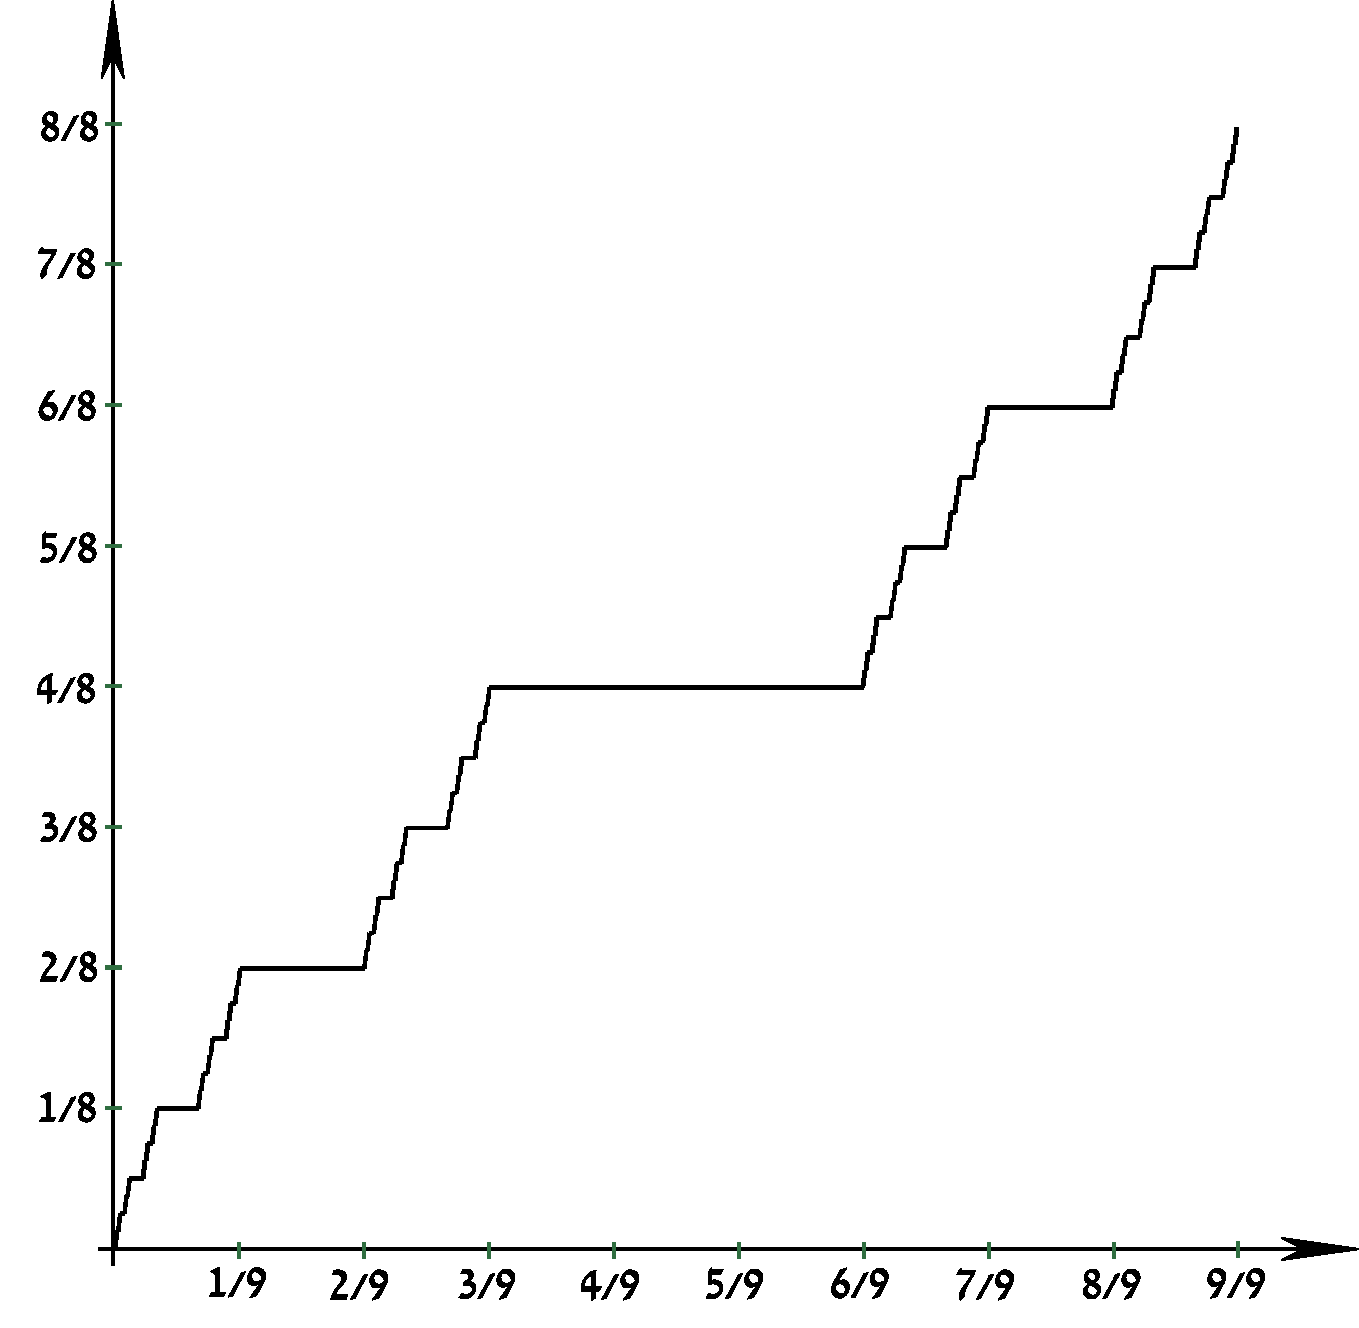
\includegraphics[width=6cm]{attachment/CantorEscalier-2.pdf}
	\caption{Cantor函数在$[0,1]$的图像, “魔鬼阶梯”}
\end{figure}

\circled{A2}-1~~验证Cantor函数在$[0,1]$上连续, 在且仅在$\mathcal{C}$以外可微, 且导数值为$0$. 

\circled{A2}-2~~称一个函数$f$在$[a,b]$上是\textit{绝对连续的}, 如果对任意$\varepsilon >0$存在$\delta >0$使得有限个不交的开区间$(a_k,b_k)$只要满足$\sum_k (b_k-a_k) <\delta$就有$\sum_k |f(b_k)-f(a_k)|<\varepsilon$.\footnote{如果将Newton-Leibniz公式中的Riemann积分替换为Lebesgue积分, 则一个函数符合该公式当且仅当其绝对连续. } 验证Cantor函数在$[0,1]$上并非绝对连续. 

\circled{A2}-3~~求$\int_0^1 c(x) \dif x$. 
\vspace{1em}

\subsection*{B: 积分相关问题}

\circled{B1}-1~~证明: 若$f \in C([a,b])$, 在$[a,b]$上非负, 则$\displaystyle \lim_{n\to \infty} \left( \int_a^b (f(x))^n \dif x \right)^{\frac{1}{n}} = \max_{a \leq x \leq b} f(x).$

\circled{B1}-2~~若$f,\varphi \in C([a,b])$在$[a,b]$上非负, 则$\displaystyle \lim_{n\to \infty} \left( \int_a^b \varphi (x) (f(x))^n \dif x \right)^{\frac{1}{n}} = \max_{a \leq x \leq b} f(x).$

\circled{B1}-3~~若$f \in C([a,b])$, 在$[a,b]$上非负, 证明: $$\lim_{n\to \infty} \left( \left( \int_a^b (f(x))^{n+1} \dif x \right) / \left( \int_a^b (f(x))^n \dif x \right) \right) = \max_{a \leq x \leq b} f(x).$$

将离散的不等式推广: 
\vspace{1em}

\circled{B2}-1~~(Jensen不等式) 设$f,g \in C(\R)$, 且$f$是凸函数, 则当$c \neq 0$时$$f\left( \frac{1}{c} \int_0^c \varphi (t) \dif t \right) \leq \frac{1}{c} \int_0^c f(\varphi (t)) \dif t.$$

\circled{B2}-2~~(Young不等式) 设实数$a,b>0$, 函数$f$在$[a,+\infty )$上连续且严格单调递增, $f(0)=0$, 则$$ab \leq \int_0^a f(x) \dif x + \int_0^b f^{-1}(x) \dif x \leq bf^{-1}(b) + af(a)-f(a)f^{-1}(b),\qquad \textit{取等} \Leftrightarrow f(a)=b.$$

\circled{B2}-3~~(Hölder不等式) 设$\frac{1}{p}+\frac{1}{q}=1$, $f,g$在$[a,b]$上Riemann可积. 则当$p > 1$时有$$\left| \int_a^b f(x)g(x) \dif x \right|\leq \left( \int_a^b |f(x)|^p \dif x \right)^{\frac{1}{p}} \left( \int_a^b |g(x)|^q \dif x \right)^{\frac{1}{q}}  ,\qquad \textit{取等}\Leftrightarrow |f|^p=\lambda |g|^q. $$
当$0<p<1$时上述不等式反向. 取$p=q=2$, 即得Cauchy-Schwarz不等式. 
\vspace{1em}

\circled{B2}-4~~(Kantorovich不等式) 设$f$在$[0,1]$上Riemann可积, 记$0<m \leq f(x) \leq M$, 则有$$\left( \int_0^1 f(x) \dif x \right) \left( \int_0^1 \frac{1}{f(x)} \dif x \right) \leq \frac{(m+M)^2}{4mM}.$$


\circled{B2}-5~~(Minkowski不等式) 设$f,g$在$[a,b]$上Riemann可积. 当$p \geq 1$时有$$\left( \int_a^b |f(x)+g(x)|^p \dif x \right)^{\frac{1}{p}} \leq \left( \int_a^b |f(x)|^p \dif x \right)^{\frac{1}{p}} + \left( \int_a^b |g(x)|^q \dif x \right)^{\frac{1}{q}},\qquad \textit{取等}\Leftrightarrow |f|^p=\lambda |g|^q.$$
当$0<p<1$时上述不等式反向. 




\newpage
\section*{一些习题 ~~\small 对应原书6.3习题} \label{sec:ex7.2}

\subsection*{A: 积分中值定理应用}

\circled{A1}~~设$f \in C(\R)$, 则对任何闭区间$[a,b]$, 任取$\varepsilon >0$均存在$\delta >0$使得$\displaystyle \left| \int_{x-\delta}^{x+\delta} f(x) \dif x-f(x) \right|<\varepsilon$. 
\vspace{1em}

\circled{A2}-1~~验证当$x \to \infty$时, 函数$f(x)=\int_{x}^{x+1} \sin t^2 \dif t$可表示为$$f(x)=\frac{\cos x^2}{2x}-\frac{\cos ((x+1)^2)}{2(x+1)}+O\left( \frac{1}{x^2} \right).$$

\circled{A2}-2~~求$\liminf_{x\to \infty} xf(x)$和$\limsup_{x \to \infty} xf(x)$. 
\vspace{1em}

设$f:[a,b] \to \R$, $\xi _1,\cdots ,\xi _m$是该区间上的不同点. 回忆Lagrange插值多项式$$L_{m-1}:=\sum_{j=1}^{m}f(\xi _j) \prod_{i \neq j} \frac{x-\xi _j}{\xi _j-\xi _i}.$$
进一步, 由\ref{sec:ex6.2}的A5-2可知若$f \in C^{m}([a,b])$, 则有$$f(x)-L_{m-1}(x)=\frac{1}{m!}f^{(m)}(\zeta (x))\omega _m(x),$$
其中$\omega _m(x)=\prod_{i=1}^{m}(x-\xi _i)$, $\zeta (x) \in (a,b)$. 作换元$\xi _i = \frac{b+a}{2} + \frac{b-a}{2} \theta _i$, 这里$\theta _i \in [-1,1]$. 
\vspace{1em}

\circled{A3}-1~~证明: $$\int_a^b L_{m-1}(x) \dif x = \frac{b-a}{2} \sum_{i=1}^{m}c_if(\xi _i),\qquad \textit{此处}~c_i=\int_{-1}^{1} \left( \prod_{j \neq i} \frac{t-\theta _i}{\theta _j - \theta _i} \right) \dif t.$$
特别地, 
\begin{itemize}
	\item 矩形: $\displaystyle \int_a^b L_0 (x) \dif x = (b-a)f\left( \frac{a+b}{2} \right)$. 
	\item 梯形: $\displaystyle \int_a^b L_1(x) \dif x = \frac{b-a}{2}(f(a)+f(b))$. 
	\item 抛物线: $\displaystyle \int_a^b L_2(x) \dif x = \frac{b-a}{6}\left( f(a)+4f\left( \frac{a+b}{2} \right) + f(b) \right)$. 
\end{itemize}
\vspace{1em}

\circled{A3}-2~~设$f \in C^m([a,b])$, 取$M_m = \sup_{x \in [a,b]} |f^{(m)}(x)|$, 令$$R_m:=\int_a^b f(x) \dif x - \int_a^b L_{m-1}(x) \dif x.$$
证明$|R_m| \leq \frac{M_m}{m!}\int_a^b |\omega _m(x)| \dif x$. 
\vspace{1em}

\circled{A3}-3~~在A3-1的三个推论中, 分别有$$R_1 = \frac{f'(\xi _1)}{4}(b-a)^2,\qquad R_2 = -\frac{f''(\xi _2)}{12}(b-a)^3 ,\qquad R_3=-\frac{f^{(4)}(\xi _3)}{2880}(b-a)^5,$$
其中$\xi _i \in [a,b]$, $f$承A3-2的定义. 
\vspace{1em}

\circled{A3}-3~~设$h=\frac{b-a}{n}$, $x_k=a+hk, y_k=f(x_k)~(k=0,\cdots ,n)$. 考虑如下余项: 
\begin{itemize}
	\item 矩形: $\displaystyle \int_a^b f(x) \dif x = h(y_0+\cdots +y_{n-1}) + R_1$. 
	\item 梯形: $\displaystyle \int_a^b f(x) \dif x = \frac{h}{2}((y_0+y_n)+2(y_1+\cdots +y_{n-1})) + R_2$. 
	\item 抛物线(Simpson): $\displaystyle \int_a^b f(x) \dif x = \frac{h}{3}((y_1+y_n)+4(y_1+y_3+\cdots +y_{n-1})+2(y_2+y_4+\cdots +y_{n-2})$, 其中$n$为偶数. 
\end{itemize}
给出$R_1,R_2,R_3$的值. 
\vspace{1em}

\circled{A3}-4~~利用上述公式, 计算$\displaystyle \pi = 4\int_0^1 \frac{\dif x}{1+x^2}$, 精确到$10^{-3}$. 


\newpage
\section{有向可加函数与Stieltjes积分}

将Riemann积分算子的区间可加性抽象出来, 得到所谓可加函数. 即, 设$I:U \times U \to V$, 若对任意$x,y,z \in U$都有$I(x,z)=I(x,y)+I(y,z)$, 则称$I$为$U$上的\textit{有向可加函数}. 这里用一般的$U,V$是为了强调有向可加函数的性质与$\R$的特殊结构无关. 

实际上, 除了Riemann积分以外, 很多函数都是有向可加函数. 例如, 向量的加法运算$\xl{AC}=\xl{AB}+\xl{BC}$, 电势差$\varphi _{ac}=\varphi _{ab}+\varphi _{bc}$等等. 不难发现, 电势差$\varphi _{ab}$的背后是场强的(多元函数)积分$\int_a^b E(r) \dif r$, 但是向量加法背后并没有明显的积分背景. 这一现象提示我们研究, 何种有向可加函数能表示为Riemann积分? 更进一步, 注意到有些离散情况的公式和积分公式非常相似(如Abel变换和分部积分), 那么可否发展一种积分理论将这些公式统一起来? 

在第一小节, 我们会探讨哪些函数能表示为Riemann积分(毕竟这种积分易于计算)及其计算. 而作为推广的Stieltjes积分将在第二小节介绍. 

\subsection{有向可加函数的Riemann积分表示}

我们可以从积分的性质反过来思考何种有向可加函数无法用积分表示. 区间可加性是自然满足的; 由于我们只想让它表示为特定函数的积分, 那些涉及多个函数的性质(线性, 保序性)不在考虑范围内. 于是只剩下估计性质, 即若$m \leq f(x) \leq M$则$m(b-a) \leq \int_a^b f(x) \leq M(b-a)$. 我们不难发现, 若将其加强为对任意子区间$[\alpha ,\beta]$均成立, 这就变成一个充分条件了. 

\begin{proposition}{}
	设有向可加函数$I:[a,b] \times [a,b] \to \R$. 若存在$f \in \mathcal{R}([a,b])$使得对任意$a \leq \alpha < \beta \leq b$都有$$\inf_{x\in [\alpha ,\beta]} f(x) (\beta -\alpha) \leq I(\alpha ,\beta) \leq \sup_{x\in [\alpha ,\beta]} f(x) (\beta -\alpha),$$
	则$\displaystyle I(a,b)=\int_a^b f(x) \dif x$. 
\end{proposition}
\begin{proof}
	应用Darboux上下和即可. 
\end{proof}

第一个例子是空间曲线(道路)的长度. 我们称一个$C^{n}$的映射$\gamma :[a,b] \to \R ^n$为$C^{n}$的\textit{曲线}(道路). 需要注意, 这条曲线并非一定是我们想象中的一条“线”, 例如Peano曲线实际填满了$[0,1]^2$. 

现在来考虑曲线的长度$I(\gamma (a) ,\gamma (b))$(这里, 我们要求两条曲线首尾相接之后在其连接点仍然是$C^n$的), 容易猜到长度应当对应速度绝对值$|\gamma '|$的积分. 实际上, 由于我们用绝对值将向量值函数转化为实值函数, 这里可以进行大小比较, 即$\int_{a}^{b} |\gamma '(t)| \dif t = |\gamma '(\xi)| (b-a)$总是介于$|\gamma '(t)| (b-a)$的下确界与上确界之间. 由上方的命题这一定义是合理的. 

\begin{remark}
	值得注意的一个事实是, 无论用何种方式\textit{参数化}曲线(即将曲线表示为上述形式的$\gamma$的值域), 计算得到的长度应当相等(良定义). 这由Riemann积分的换元公式立刻可以得到. 
\end{remark}}

第二个例子在前文已经提到过, 即向量的加法运算$\xl{AC}=\xl{AB}+\xl{BC}$. 实际上, 作为有向可加函数, 它的运算结果不是一维的实数, 而是更高维的向量, 这就导致上方的不等式无法定义. 更进一步, 由于$\R ^n$无法被赋予全序结构, 不管采用何种高维推广的定义都会有例外的向量. 由此, 我们就从代数的角度解释了几何上的直观(即其无法被定义为积分). 

\subsection{Stieltjes积分}

对于有向可加函数$I:[a,b] \times [a,b] \to \R$, 通过定义函数$\mu :[a,b] \to \R ,t \mapsto I(a,t)$, 可将$I(\alpha ,\beta)$视作$\mu (\beta)-\mu (\alpha)$. 从几何的视角, 若将$I(\alpha ,\beta)$视作区间$[\alpha ,\beta ]$的长度(两端点的有向距离), 则$\mu$就给出了某个点的绝对位置(亦称$\mu$为测度函数). Riemann积分即是$\mu (x)=x$的情形. 这启发我们, 将Riemann积分中的$\dif x$替换为$\dif \mu (x)$, 或者说将Riemann和中的$x_i-x_{i-1}$替换为$\mu (x_i)- \mu (x_{i-1})$. 

需要注意的是, 虽然$\mu $的单调性不影响Stieltjes积分的定义(类似换元积分公式不要求$\varphi$单调), 但为了得到更有用的命题, 会约定$\mu$不减. 

\begin{definition}{Stieltjes积分}
	设闭区间$I$上的函数$f$和不减的函数$\mu$, 定义
	\begin{itemize}
		\item 对于分划$\pi = \{ a=x_0<\cdots <x_n=b \}$, 称形如$$f = \sum_{i=1}^{n} \lambda _i \chi _{(\mu (x_{i-1}),\mu (x_{i}))} $$
		(其中$\lambda _i \in \R$)的函数为$\pi$上的一个\textit{$\mu$-阶梯函数}. 记$I$上全体$\mu$-阶梯函数的集合为$\mathcal{S}(I;\mu )$. 
		\item 承上一条, 定义$f$的\textit{积分}(integral)为$$\int f := \sum_{i=1}^{n} \lambda _i \int \chi _{(\mu (x_{i-1}), \mu (x_i))} = \sum_{i=1}^{n} \lambda _i (\mu (x_i)-\mu (x_{i-1})). $$
		\item 称$f$是\textit{Stieltjes可积的}, 如果对任意$\varepsilon >0$均存在$F,e \in \mathcal{S}(I;\mu )$使得$$\forall x \in I,|f(x)-F(x)|<e(x),\qquad \int e < \varepsilon .$$
	全体$I$上Riemann可积的函数构成集合$\mathcal{R}(I;\mu)$. 
	\end{itemize}
	类似Riemann积分, 我们还能验证Riemann和的定义与上方定义等价: 
	\begin{itemize}
		\item $f$的\textit{Riemann和}为$$S(f;\pi ,\xi) := \sum_{i=1}^{n} (\mu(x_i)-\mu(x_{i-1}))f(\xi _i) .$$
		\item 固定$f$, 它的\textit{基}为$\mathcal{B} := \{ B_{\delta}:\delta >0 \}$, 其中$B_{\delta} := \{ (\pi ,\xi) : \| \pi \|< \delta \}$. 
		\item 称$f$在$I$上\textit{Stieltjes可积}, 若极限$\displaystyle \lim_{\mathcal{B}} S(f;\pi ,\xi)$存在, 且将其定义为$\displaystyle \int_a^b f(x) \dif \mu (x)$. 
	\end{itemize}
\end{definition}

同样地, 对阶梯函数与Riemann和而言, 分别可以定义上下积分及Darboux上下和. 这里省略具体定义. 

可以证明Stieltjes积分拥有和Riemann积分类似的性质, 即命题\ref{pro:jiffxkvi1}(注意保序性依赖$\mu$不减), \ref{pro:kejiisyc}(要将$x$换成$\mu (x)$), \ref{pro:jiffxkvi}. 

类似于换元积分公式, 不难证明, 设$\mu (x) = \int_a^x \rho (x)\dif x$, 则对可积的$f$有$\displaystyle \int_a^b f(x) \dif \mu (x) = \int_a^b f(x) \rho (x) \dif x$. 特别地, 当$\mu$连续可微时, 就可以将积分号内的$\dif \mu (x)$看做是$\mu '(x) \dif x$. 

然而, 唯一与Riemann积分不同之处在于, Stieltjes积分没有Newton-Leibniz公式. 这是否意味着其没有作为Newton-Leibniz公式推论的分部积分公式? 实际上, 用Abel求和来逼近, 可以证明类似分部积分的公式. 

\begin{proposition}{分部积分公式}
	设$f \in C^1([a,b])$, 则$$\int_a^b f'(x)\mu (x) \dif x = (f(x)\mu (x)) |_a^b - \int_a^b f(x) \dif \mu (x) .$$
\end{proposition}
\begin{proof}
	对于分割$\pi$, 由Lagrange中值定理, 存在$\xi _i \in (x_{i-1},x_i)$使得$f(x_i)-f(x_{i-1})=f'(\xi _i)(x_i-x_{i-1})$. 易得(但不显然)下式成立: $$\left| \sum_{\pi} f'(\xi _i)\mu (x_i)(x_i-x_{i-1})-\int_a^b f'(x) \mu (x) \dif x \right| \to 0,\quad \| \pi \| \to 0. $$
	对$\sum_{\pi} f'(\xi _i)\mu (x_i)(x_i-x_{i-1})$作Abel变换, 我们有
	\begin{align*}
		\sum_{i=1}^{n} f'(\xi _i)\mu (x_i)(x_i-x_{i-1}) &= \sum_{i=1}^{n} \mu (x_i)(f(x_i)-f(x_{i-1})) \\
		&= \mu (x_n)(f(x_n)-f(x_0)) - \sum_{i=1}^{n-1} (f(x_i)-f(x_0))(\mu (x_{i+1})-\mu (x_i)) \\
		&= (f(x)\mu (x))|_a^b - \sum_{i=0}^{n-1} f(x_i)(\mu (x_{i+1})-\mu (x_i)). 
	\end{align*}
	令$\| \pi \|\to 0$即可. 
\end{proof}

利用Stieltjes积分, 可以得到(弱形式)第二积分中值定理的另一个证明: 

\begin{example}
	设$f \in C([a,b])$, $g \in \mathcal{R}([a,b])$, $g$是单调不增的非负函数, 则存在$\xi \in [a,b]$使得$\displaystyle \int_a^b f(x) g(x) \dif x = g(a) \int_a^{\xi} f(x) \dif x.$
\end{example}
\begin{proof}
	令$F(x)=\int_a^x f(t) \dif t$, 则$F$连续可微. 记$m \leq F(x) \leq M$, 则$$\int_a^b f(x)g(x) \dif x = F(b)g(b) + \int_a^b F(x)\dif (-g)(x) \leq F(b)g(b)+M\int_a^b \dif (-g)(x) \leq Mg(a).$$
	同理$\int_a^b f(x)g(x) \dif x \geq mg(a)$, 由$F$连续立得原命题成立. 
\end{proof}

Stieltjes积分的一大应用在于将求和与积分的互相转化. 接下来我们着重介绍这部分内容. 我们先考虑最基础(无脑)的方法: 

\begin{lemma}{}
	设数列$\{ a_n \}$, 若函数$f$满足$f|_{[k-1,k)}=a_k$, 则$\sum_{n<k\leq m} a_k = \int_n^m f(x) \dif \qz{x}$. 
\end{lemma}
\begin{remark}
	条件可减弱为$f(k^-)=a_k$. 
\end{remark}
\begin{proof}
	用Riemann和的形式写出$\int_n^m f(x) \dif \qz{x}=\sum _{\pi} f(\xi _i)(\qz{x_i}-\qz{x_{i-1}})$. 容易发现只有使得$x_{i-1}<k\leq x_i$的项有所贡献, 其中$k$是某整数. 因此上式最终变成了$\sum_{k=n+1}^{m} f(\xi _k) (k-(k-1))$, 这里$k-1 \leq \xi _k < k$. 显然$f(\xi _k)=a_k$, 这就证明了引理. 
\end{proof}

这个引理只能应用到一元求和. 对于多重求和, 我们有类似的结论: 

\begin{lemma}{}
	设数列$\{ a_{i_1,\cdots ,i_n} \}$, 若函数$f$满足$f|_{[i_1-1,i_1) \times \cdots \times [i_n-1,i_n)}=a_{i_1,\cdots ,i_n}$, 则$$\sum_{\alpha _1 < i_1 \leq \beta _1 ,\cdots ,\alpha _n< i_n \leq \beta _n} a_{i_1,\cdots ,i_n} = \int_{(\alpha _1,\beta _1]\times \cdots \times (\alpha _n,\beta _n]} f(x) \dif \qz{x}.$$
	其中, $x \in \R ^n$且$\qz{x}:=(\qz{x^1},\cdots ,\qz{x^n})$. 
\end{lemma}
\begin{remark}
	条件可减弱为$f((i_1,\cdots ,i_n)^-)=a_{i_1,\cdots ,i_n}$. 
\end{remark}

在实际情景中, 不一定求和范围就是一个标准的方块形, 此时可参考下例解决. 

\begin{example}
	求所有的实数$\alpha$使得$\displaystyle \lim_{r \to \infty} \sum_{0<\| v \|_2 < R ,v \in \Z ^3} \| v \|_2 ^{\alpha}$存在且有限. \footnote{题源\textit{2023年10月清华领军计划一试第4题}; 解答来自数之谜用户\textit{对吧}. }
\end{example}
\begin{solution}
	记$v=(x,y,z)$. 令$\mu (r)$表示$x^2+y^2+z^2<r^2,x,y,z \in \Z$的解数, 于是$$\sum_{0<\| v \|_2 < R ,v \in \Z ^3} \| v \|_2 ^{\alpha} = \int_0^{\sqrt{R}} t^{\alpha} \dif \mu (t) = (t^{\alpha} \mu (t))\big|_0^{\sqrt{R}} - \int_0^{\sqrt{R}} \alpha t^{\alpha -1} \mu (t) \dif t.$$
	我们有估计$\frac{4}{3}\pi (r-1)^3 \leq \mu (r) \leq \frac{4}{3}\pi (r+1)^3$, 因此$\mu (r) = \frac{4}{3}\pi r^3+O(r^2)$, 代入上式: $$\textit{上式}~= R^{\frac{\alpha}{2}}\left( \frac{4}{3}\pi R^{\frac{3}{2}}+O(R) \right) - \frac{4}{3}\pi \alpha \cdot \frac{1}{\alpha +3} R^{\frac{\alpha +3}{2}} + O(R^{\frac{\alpha +2}{2}}) = \frac{4\pi}{\alpha +3} R^{\frac{\alpha +3}{2}} + O(R^{\frac{\alpha +2}{2}}).$$
	因此极限存在当且仅当$\alpha <-3$. 
\end{solution}

进一步, 可以估计$\int f(x) \dif \qz{x}$与$\int f(x) \dif x$间的误差. 

\begin{proposition}{Euler–Maclaurin公式}
	设$f \in C^1([a,b])$, 则当$a$不为整数时, $$\sum_{a<k \leq b} f(k) = \int_a^b f(x) \dif x + \int_a^b f'(x)(x-\qz{x}) \dif x + f(a)(a-\qz{a})-f(b)(b-\qz{b}).$$
	当$a$为整数时, 上式的$f(a)(a-\qz{a})$变为$f(a)$. 
\end{proposition}
\begin{proof}
	当$a$不为整数时: 由分部积分公式, $$\int_a^b f(x) \dif (x-\qz{x}) + \int_a^b f'(x)(x-\qz{x}) \dif x = f(a)(a-\qz{a})-f(b)(b-\qz{b}).$$
	其中, $\int_a^b f(x) \dif (x-\qz{x}) = \int_a^b f(x) \dif x - \sum_{a<k \leq b}f(k)$. 代入上式即得. 
	
	当$a$为整数时: 将$a'=a-\varepsilon ,0<\varepsilon <1$代入上一情形, 此时$f(a')(a'-\qz{a'}) = f(a-\varepsilon)(1-\varepsilon)$. 令$\varepsilon \to 0^+$即得. 
\end{proof}

\begin{example}
	求$\displaystyle \sum_{n=1}^{\infty} (-1)^{n-1} \frac{\ln n}{n}$. 
\end{example}
\begin{solution}
	由交错级数的命题, 原式收敛. 容易发现$$\sum_{n=1}^{2N} (-1)^{n-1} \frac{\ln n}{n} = \sum_{n=1}^{2N} \frac{\ln n}{n} - 2\sum_{n=1}^{N} \frac{\ln 2n}{2n} = \sum_{n=N+1}^{2N} \frac{\ln n}{n} - \ln 2 \sum_{n=1}^{N} \frac{1}{n} .$$
	因此只需处理$\sum_{n=N+1}^{2N} \frac{\ln n}{n}$. 实际上, 首先计算$\int_N^{2N} \frac{\ln x}{x} \dif x = \frac{1}{2}((\ln 2N)^2-(\ln N)^2) = \frac{\ln 2}{2}\ln (2N^2) $, 接下来估计误差: 
	\begin{align*}
		\left| \sum_{n=N+1}^{2N} \frac{\ln n}{n} - \frac{\ln 2}{2}\ln (2N^2) \right| &\leq \left| \int_{N}^{2N} (x-\qz{x}) \frac{1-\ln x}{x^2} \dif x \right| + \left| \frac{\ln N}{N} \right| \\
		&\leq \left| \frac{\ln 2N}{2N} \right| + 2\left| \frac{\ln N}{N} \right| \to 0,\quad N \to \infty .
	\end{align*}
	于是$$\textit{原式} = \lim_{N \to \infty} \sum_{n=1}^{2N} (-1)^{n-1} \frac{\ln n}{n} = \lim_{N \to \infty} \frac{\ln 2}{2}\ln (2N^2) - \ln 2\sum_{n=1}^{N} \frac{1}{n} = \frac{(\ln 2)^2}{2} - \gamma \ln 2.$$
	其中$\gamma$是Euler常数. 
\end{solution}

除了强行以$\qz{x}$为测度函数, 我们当然有更加自由的方式: 其基本想法是将$\qz{x}$换成真正的阶梯函数. 例如, 回忆Abel求和公式: $\sum_{n=1}^{N} a_nb_n = S_Nb_N - \sum_{n=1}^{N-1} S_n(b_{n+1}-b_n)$. 实际上, 令$f' = \sum_{n=1}^{N} a_n \chi_{[n,n+1 )}$, 从而$f = \sum_{n=1}^{N} S_n\chi_{[n,n+1 )}$. 再令$\mu = \sum_{n=1}^{N} b_n \chi_{[n,n+1 )}$. 于是我们有$$\sum_{n=1}^{N} a_nb_n = \int_1^N f' \mu = f\mu \big|_1^N - \int_1^N f \dif \mu = S_Nb_N - \sum_{n=1}^{N-1} S_n(b_{n+1}-b_n). $$

最后一种转化方法暂时难以举出典型用例, 读者可查阅Lebesgue-Stieltjes积分内容找到例子(因为这种方法的核心Dirac函数有着明显的测度意义). 

\begin{example}
	(Heaviside函数)~设$f:[a,b] \to \R$有界且在$c$处连续. 令$\mu _c=\chi _{[c,b]}$. 则$\displaystyle \int_a^b f \dif \mu _c = f(c)$. 
\end{example}
\begin{remark}
	所谓的Dirac(广义)函数定义为$\delta (x) = \begin{cases}
		+\infty & x=c \\ 0 & x \neq c
	\end{cases}$且$\int_a^b \delta (x) =1$. 注意到, Heaviside函数就是其某种意义上的积分. 这一点参考附录. 
\end{remark}
\begin{proof}
	由$f$在$c$处连续不难证明该积分值存在. 不难发现$\int_a^b f \dif \mu _c = f(c)(\mu (c^+)- \mu (c^-)) = f(c)$. 
\end{proof}






由Heaviside函数的例子, 不难得到下方引理: 

\begin{lemma}{}
	设正实数列$\{ a_n \}$且$\sum_{n=1}^{\infty} a_n$收敛, $\{ x_n \}\subseteq (a,b)$. 令$\mu = \sum_{i=1}^{\infty} a_i\chi _{[x_i,+\infty)}$, 则对连续函数$f$有$\int_a^b f \dif \mu = \sum_{i=1}^{\infty} a_if(x_i)$. 
\end{lemma}
\begin{proof}
	由级数收敛, 任取$\varepsilon$都存在$N>0$使得$\sum_{N+1}^{\infty} a_n <\varepsilon$. 取$f$的一个上界$M$, 由Dirac函数可知
	\begin{align*}
		\left| \int_a^b f \dif \mu - \sum_{i=1}^{\infty} a_if(x_i) \right| &= \left| \int_a^b f \dif (\mu|_{\geq N+1}) - \sum_{i=N+1}^{\infty} a_if(x_i) \right| \\
		&\leq M|(\mu|_{\geq N+1})|_a^b| + M\varepsilon \leq (1+a+b)M\varepsilon .
	\end{align*}
	由$\varepsilon$的任意性即得. 
\end{proof}























